


%% bare_conf.tex
%% V1.3
%% 2007/01/11
%% by Michael Shell
%% See:
%% http://www.michaelshell.org/
%% for current contact information.
%%
%% This is a skeleton file demonstrating the use of IEEEtran.cls
%% (requires IEEEtran.cls version 1.7 or later) with an IEEE conference paper.
%%
%% Support sites:
%% http://www.michaelshell.org/tex/ieeetran/
%% http://www.ctan.org/tex-archive/macros/latex/contrib/IEEEtran/
%% and
%% http://www.ieee.org/

%%*************************************************************************
%% Legal Notice:
%% This code is offered as-is without any warranty either expressed or
%% implied; without even the implied warranty of MERCHANTABILITY or
%% FITNESS FOR A PARTICULAR PURPOSE! 
%% User assumes all risk.
%% In no event shall IEEE or any contributor to this code be liable for
%% any damages or losses, including, but not limited to, incidental,
%% consequential, or any other damages, resulting from the use or misuse
%% of any information contained here.
%%
%% All comments are the opinions of their respective authors and are not
%% necessarily endorsed by the IEEE.
%%
%% This work is distributed under the LaTeX Project Public License (LPPL)
%% ( http://www.latex-project.org/ ) version 1.3, and may be freely used,
%% distributed and modified. A copy of the LPPL, version 1.3, is included
%% in the base LaTeX documentation of all distributions of LaTeX released
%% 2003/12/01 or later.
%% Retain all contribution notices and credits.
%% ** Modified files should be clearly indicated as such, including  **
%% ** renaming them and changing author support contact information. **
%%
%% File list of work: IEEEtran.cls, IEEEtran_HOWTO.pdf, bare_adv.tex,
%%                    bare_conf.tex, bare_jrnl.tex, bare_jrnl_compsoc.tex
%%*************************************************************************

% *** Authors should verify (and, if needed, correct) their LaTeX system  ***
% *** with the testflow diagnostic prior to trusting their LaTeX platform ***
% *** with production work. IEEE's font choices can trigger bugs that do  ***
% *** not appear when using other class files.                            ***
% The testflow support page is at:
% http://www.michaelshell.org/tex/testflow/



% Note that the a4paper option is mainly intended so that authors in
% countries using A4 can easily print to A4 and see how their papers will
% look in print - the typesetting of the document will not typically be
% affected with changes in paper size (but the bottom and side margins will).
% Use the testflow package mentioned above to verify correct handling of
% both paper sizes by the user's LaTeX system.
%
% Also note that the "draftcls" or "draftclsnofoot", not "draft", option
% should be used if it is desired that the figures are to be displayed in
% draft mode.
%
\documentclass[10pt, conference, compsocconf]{IEEEtran}
% Add the compsocconf option for Computer Society conferences.
%
% If IEEEtran.cls has not been installed into the LaTeX system files,
% manually specify the path to it like:
% \documentclass[conference]{../sty/IEEEtran}

\usepackage[brazil]{babel}
\usepackage[latin1]{inputenc}



% Some very useful LaTeX packages include:
% (uncomment the ones you want to load)


% *** MISC UTILITY PACKAGES ***
%
%\usepackage{ifpdf}
% Heiko Oberdiek's ifpdf.sty is very useful if you need conditional
% compilation based on whether the output is pdf or dvi.
% usage:
% \ifpdf
%   % pdf code
% \else
%   % dvi code
% \fi
% The latest version of ifpdf.sty can be obtained from:
% http://www.ctan.org/tex-archive/macros/latex/contrib/oberdiek/
% Also, note that IEEEtran.cls V1.7 and later provides a builtin
% \ifCLASSINFOpdf conditional that works the same way.
% When switching from latex to pdflatex and vice-versa, the compiler may
% have to be run twice to clear warning/error messages.






% *** CITATION PACKAGES ***
%
%\usepackage{cite}
% cite.sty was written by Donald Arseneau
% V1.6 and later of IEEEtran pre-defines the format of the cite.sty package
% \cite{} output to follow that of IEEE. Loading the cite package will
% result in citation numbers being automatically sorted and properly
% "compressed/ranged". e.g., [1], [9], [2], [7], [5], [6] without using
% cite.sty will become [1], [2], [5]--[7], [9] using cite.sty. cite.sty's
% \cite will automatically add leading space, if needed. Use cite.sty's
% noadjust option (cite.sty V3.8 and later) if you want to turn this off.
% cite.sty is already installed on most LaTeX systems. Be sure and use
% version 4.0 (2003-05-27) and later if using hyperref.sty. cite.sty does
% not currently provide for hyperlinked citations.
% The latest version can be obtained at:
% http://www.ctan.org/tex-archive/macros/latex/contrib/cite/
% The documentation is contained in the cite.sty file itself.






% *** GRAPHICS RELATED PACKAGES ***
%
\ifCLASSINFOpdf
  \usepackage[pdftex]{graphicx}
  % declare the path(s) where your graphic files are
  % \graphicspath{{../pdf/}{../jpeg/}}
  % and their extensions so you won't have to specify these with
  % every instance of \includegraphics
  \DeclareGraphicsExtensions{.pdf,.jpeg,.png}
\else
  % or other class option (dvipsone, dvipdf, if not using dvips). graphicx
  % will default to the driver specified in the system graphics.cfg if no
  % driver is specified.
  \usepackage[dvipdfm]{graphicx}
  % declare the path(s) where your graphic files are
  % \graphicspath{{../eps/}}
  % and their extensions so you won't have to specify these with
  % every instance of \includegraphics
  \DeclareGraphicsExtensions{.eps}
\fi
% graphicx was written by David Carlisle and Sebastian Rahtz. It is
% required if you want graphics, photos, etc. graphicx.sty is already
% installed on most LaTeX systems. The latest version and documentation can
% be obtained at: 
% http://www.ctan.org/tex-archive/macros/latex/required/graphics/
% Another good source of documentation is "Using Imported Graphics in
% LaTeX2e" by Keith Reckdahl which can be found as epslatex.ps or
% epslatex.pdf at: http://www.ctan.org/tex-archive/info/
%
% latex, and pdflatex in dvi mode, support graphics in encapsulated
% postscript (.eps) format. pdflatex in pdf mode supports graphics
% in .pdf, .jpeg, .png and .mps (metapost) formats. Users should ensure
% that all non-photo figures use a vector format (.eps, .pdf, .mps) and
% not a bitmapped formats (.jpeg, .png). IEEE frowns on bitmapped formats
% which can result in "jaggedy"/blurry rendering of lines and letters as
% well as large increases in file sizes.
%
% You can find documentation about the pdfTeX application at:
% http://www.tug.org/applications/pdftex





% *** MATH PACKAGES ***
%
%\usepackage[cmex10]{amsmath}
% A popular package from the American Mathematical Society that provides
% many useful and powerful commands for dealing with mathematics. If using
% it, be sure to load this package with the cmex10 option to ensure that
% only type 1 fonts will utilized at all point sizes. Without this option,
% it is possible that some math symbols, particularly those within
% footnotes, will be rendered in bitmap form which will result in a
% document that can not be IEEE Xplore compliant!
%
% Also, note that the amsmath package sets \interdisplaylinepenalty to 10000
% thus preventing page breaks from occurring within multiline equations. Use:
%\interdisplaylinepenalty=2500
% after loading amsmath to restore such page breaks as IEEEtran.cls normally
% does. amsmath.sty is already installed on most LaTeX systems. The latest
% version and documentation can be obtained at:
% http://www.ctan.org/tex-archive/macros/latex/required/amslatex/math/





% *** SPECIALIZED LIST PACKAGES ***
%
%\usepackage{algorithmic}
% algorithmic.sty was written by Peter Williams and Rogerio Brito.
% This package provides an algorithmic environment fo describing algorithms.
% You can use the algorithmic environment in-text or within a figure
% environment to provide for a floating algorithm. Do NOT use the algorithm
% floating environment provided by algorithm.sty (by the same authors) or
% algorithm2e.sty (by Christophe Fiorio) as IEEE does not use dedicated
% algorithm float types and packages that provide these will not provide
% correct IEEE style captions. The latest version and documentation of
% algorithmic.sty can be obtained at:
% http://www.ctan.org/tex-archive/macros/latex/contrib/algorithms/
% There is also a support site at:
% http://algorithms.berlios.de/index.html
% Also of interest may be the (relatively newer and more customizable)
% algorithmicx.sty package by Szasz Janos:
% http://www.ctan.org/tex-archive/macros/latex/contrib/algorithmicx/




% *** ALIGNMENT PACKAGES ***
%
%\usepackage{array}
% Frank Mittelbach's and David Carlisle's array.sty patches and improves
% the standard LaTeX2e array and tabular environments to provide better
% appearance and additional user controls. As the default LaTeX2e table
% generation code is lacking to the point of almost being broken with
% respect to the quality of the end results, all users are strongly
% advised to use an enhanced (at the very least that provided by array.sty)
% set of table tools. array.sty is already installed on most systems. The
% latest version and documentation can be obtained at:
% http://www.ctan.org/tex-archive/macros/latex/required/tools/


%\usepackage{mdwmath}
%\usepackage{mdwtab}
% Also highly recommended is Mark Wooding's extremely powerful MDW tools,
% especially mdwmath.sty and mdwtab.sty which are used to format equations
% and tables, respectively. The MDWtools set is already installed on most
% LaTeX systems. The lastest version and documentation is available at:
% http://www.ctan.org/tex-archive/macros/latex/contrib/mdwtools/


% IEEEtran contains the IEEEeqnarray family of commands that can be used to
% generate multiline equations as well as matrices, tables, etc., of high
% quality.


%\usepackage{eqparbox}
% Also of notable interest is Scott Pakin's eqparbox package for creating
% (automatically sized) equal width boxes - aka "natural width parboxes".
% Available at:
% http://www.ctan.org/tex-archive/macros/latex/contrib/eqparbox/





% *** SUBFIGURE PACKAGES ***
%\usepackage[tight,footnotesize]{subfigure}
% subfigure.sty was written by Steven Douglas Cochran. This package makes it
% easy to put subfigures in your figures. e.g., "Figure 1a and 1b". For IEEE
% work, it is a good idea to load it with the tight package option to reduce
% the amount of white space around the subfigures. subfigure.sty is already
% installed on most LaTeX systems. The latest version and documentation can
% be obtained at:
% http://www.ctan.org/tex-archive/obsolete/macros/latex/contrib/subfigure/
% subfigure.sty has been superceeded by subfig.sty.



%\usepackage[caption=false]{caption}
%\usepackage[font=footnotesize]{subfig}
% subfig.sty, also written by Steven Douglas Cochran, is the modern
% replacement for subfigure.sty. However, subfig.sty requires and
% automatically loads Axel Sommerfeldt's caption.sty which will override
% IEEEtran.cls handling of captions and this will result in nonIEEE style
% figure/table captions. To prevent this problem, be sure and preload
% caption.sty with its "caption=false" package option. This is will preserve
% IEEEtran.cls handing of captions. Version 1.3 (2005/06/28) and later 
% (recommended due to many improvements over 1.2) of subfig.sty supports
% the caption=false option directly:
%\usepackage[caption=false,font=footnotesize]{subfig}
%
% The latest version and documentation can be obtained at:
% http://www.ctan.org/tex-archive/macros/latex/contrib/subfig/
% The latest version and documentation of caption.sty can be obtained at:
% http://www.ctan.org/tex-archive/macros/latex/contrib/caption/




% *** FLOAT PACKAGES ***
%
%\usepackage{fixltx2e}
% fixltx2e, the successor to the earlier fix2col.sty, was written by
% Frank Mittelbach and David Carlisle. This package corrects a few problems
% in the LaTeX2e kernel, the most notable of which is that in current
% LaTeX2e releases, the ordering of single and double column floats is not
% guaranteed to be preserved. Thus, an unpatched LaTeX2e can allow a
% single column figure to be placed prior to an earlier double column
% figure. The latest version and documentation can be found at:
% http://www.ctan.org/tex-archive/macros/latex/base/



%\usepackage{stfloats}
% stfloats.sty was written by Sigitas Tolusis. This package gives LaTeX2e
% the ability to do double column floats at the bottom of the page as well
% as the top. (e.g., "\begin{figure*}[!b]" is not normally possible in
% LaTeX2e). It also provides a command:
%\fnbelowfloat
% to enable the placement of footnotes below bottom floats (the standard
% LaTeX2e kernel puts them above bottom floats). This is an invasive package
% which rewrites many portions of the LaTeX2e float routines. It may not work
% with other packages that modify the LaTeX2e float routines. The latest
% version and documentation can be obtained at:
% http://www.ctan.org/tex-archive/macros/latex/contrib/sttools/
% Documentation is contained in the stfloats.sty comments as well as in the
% presfull.pdf file. Do not use the stfloats baselinefloat ability as IEEE
% does not allow \baselineskip to stretch. Authors submitting work to the
% IEEE should note that IEEE rarely uses double column equations and
% that authors should try to avoid such use. Do not be tempted to use the
% cuted.sty or midfloat.sty packages (also by Sigitas Tolusis) as IEEE does
% not format its papers in such ways.





% *** PDF, URL AND HYPERLINK PACKAGES ***
%
%\usepackage{url}
% url.sty was written by Donald Arseneau. It provides better support for
% handling and breaking URLs. url.sty is already installed on most LaTeX
% systems. The latest version can be obtained at:
% http://www.ctan.org/tex-archive/macros/latex/contrib/misc/
% Read the url.sty source comments for usage information. Basically,
% \url{my_url_here}.





% *** Do not adjust lengths that control margins, column widths, etc. ***
% *** Do not use packages that alter fonts (such as pslatex).         ***
% There should be no need to do such things with IEEEtran.cls V1.6 and later.
% (Unless specifically asked to do so by the journal or conference you plan
% to submit to, of course. )


% correct bad hyphenation here
\hyphenation{op-tical net-works semi-conduc-tor}


\begin{document}
%
% paper title
% can use linebreaks \\ within to get better formatting as desired
%\title{Bare Demo of IEEEtran.cls for IEEECS Conferences / adapted for Sibgrapi 2009}
\title{Gera��o Procedural de Terrenos Pseudo-Infinitos em Tempo-Real Utilizando Arquiteturas GPU/CPU}

%------------------------------------------------------------------------- 
% change the % on next lines to produce the final camera-ready version 
\newif\iffinal
%\finalfalse
\finaltrue
\newcommand{\jemsid}{99999}
%------------------------------------------------------------------------- 

% author names and affiliations
% use a multiple column layout for up to two different
% affiliations

\iffinal
  \author
    {\IEEEauthorblockN{F�bio Markus N. Miranda, Luiz Chaimowicz}
     \IEEEauthorblockA{Departamento de Ci�ncia da Computa��o\\
						UFMG\\
						Email: fabiom@gmail.com, chaimo@dcc.ufmg.br}
  }
\else
  \author{Sibgrapi paper ID: \jemsid \\ }
\fi

% conference papers do not typically use \thanks and this command
% is locked out in conference mode. If really needed, such as for
% the acknowledgment of grants, issue a \IEEEoverridecommandlockouts
% after \documentclass

% for over three affiliations, or if they all won't fit within the width
% of the page, use this alternative format:
% 
%\author{\IEEEauthorblockN{Michael Shell\IEEEauthorrefmark{1},
%Homer Simpson\IEEEauthorrefmark{2},
%James Kirk\IEEEauthorrefmark{3}, 
%Montgomery Scott\IEEEauthorrefmark{3} and
%Eldon Tyrell\IEEEauthorrefmark{4}}
%\IEEEauthorblockA{\IEEEauthorrefmark{1}School of Electrical and Computer Engineering\\
%Georgia Institute of Technology,
%Atlanta, Georgia 30332--0250\\ Email: see http://www.michaelshell.org/contact.html}
%\IEEEauthorblockA{\IEEEauthorrefmark{2}Twentieth Century Fox, Springfield, USA\\
%Email: homer@thesimpsons.com}
%\IEEEauthorblockA{\IEEEauthorrefmark{3}Starfleet Academy, San Francisco, California 96678-2391\\
%Telephone: (800) 555--1212, Fax: (888) 555--1212}
%\IEEEauthorblockA{\IEEEauthorrefmark{4}Tyrell Inc., 123 Replicant Street, Los Angeles, California 90210--4321}}




% use for special paper notices
%\IEEEspecialpapernotice{(Invited Paper)}


%------------------------------------------------------------------------- 
% Special Sibgrapi teaser
\teaser{%
  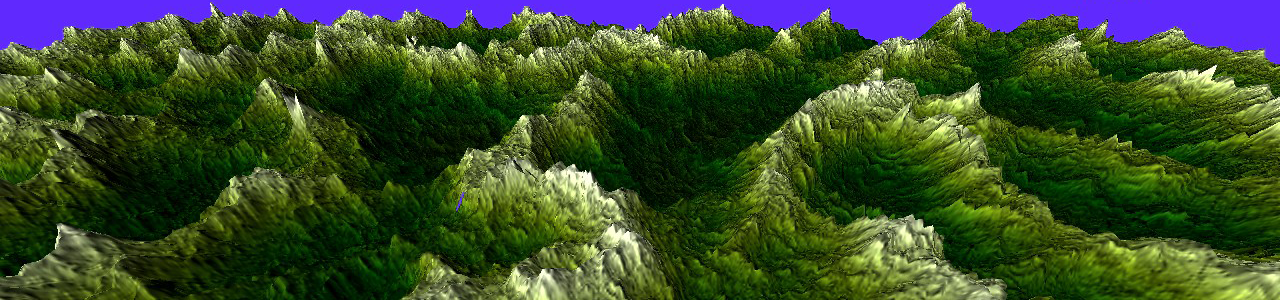
\includegraphics[width=.8\linewidth]{img/teaser.png}
  \caption{Terreno gerado proceduralmente.}
  \label{fig:teaser}
}
%------------------------------------------------------------------------- 



% make the title area
\maketitle


\begin{abstract}
O r�pido crescimento do poder de processamento das placas gr�ficas fez com que diversas tarefas migrassem da CPU para a GPU. Por�m, as unidades de processamento gr�fico podem ser vistas como aliadas da CPU, e n�o rivais. Este trabalho prop�e um modelo que utilize tanto a CPU quanto a GPU para minimizar o tempo gasto com a gera��o procedural de terrenos e permitir uma navega��o fluida atrav�s de um mundo pseudo-infinito gerado proceduralmente.

Ao final, uma discuss�o � feita com base em testes com tr�s modelos de gera��o (apenas CPU, apenas GPU, GPU e CPU), com o objetivo de expor suas vantagens e desvantagens.
\end{abstract}

\begin{IEEEkeywords}
gera��o procedural; gpu; gpgpu; programa��o paralela
\end{IEEEkeywords}


% For peer review papers, you can put extra information on the cover
% page as needed:
% \ifCLASSOPTIONpeerreview
% \begin{center} \bfseries EDICS Category: 3-BBND \end{center}
% \fi
%
% For peerreview papers, this IEEEtran command inserts a page break and
% creates the second title. It will be ignored for other modes.
\IEEEpeerreviewmaketitle




\chapter{INTRODUÇÃO}

\section{Visão geral}

    Exemplo de uso de siglas:
    
    Os modelos como \emph{Capability Maturity Model Integration} (\sigla{CMMI}{Capability Maturity Model Integration}), usado para avaliação da qualidade de \emph{software} a partir da maturidade dos processos da organização, tem ganhado muita ênfase no contexto da tecnologia de processos de \emph{software}.

    Exemplo de uso de referências:
    
    A incorporação de um processo geralmente não acontece de imediato, logo depois do processo ser formalizado. As pessoas da organização podem apresentar certa resistência quanto a mudança de hábitos, considerando os passos recomendados pelo processo apenas uma burocracia sem nenhuma vantagem para o projeto \cite{Wilson2002}. 


\section{Objetivo, justificativa e motivação}



\section{Trabalhos relacionados}
\label{trabalhosRelacionados}

A modelagem procedural de terrenos � uma �rea vastamente pesquisada, com diversos trabalhos que buscam sempre criar os terrenos mais realistas poss�veis.

Uma das t�cnicas utilizadas na modelagem procedural de terrenos � o ru�do Perlin \cite{perlinNoise}, uma fun��o pseudo-aleat�ria que, dada uma entrada (posi��o), retorna um valor que possui uma suave transi��o com os seus vizinhos. Em \cite{improvedPerlinNoise} foi apresentado um ru�do Perlin otimizado, que buscou adaptar o ru�do �s novas arquiteturas (GPUs), melhorar as propriedades visuais e introduzir uma �nica vers�o do ru�do que retornaria os mesmos valores independentemente da plataforma de \emph{hardware} ou \emph{software}.


Em \cite{proceduralApproach} s�o apresentados alguns algoritmos que fazem uso do ru�do Perlin e que s�o capazes de gerar terrenos de uma forma significativamente realista. Podemos citar os algoritmos \emph{fBm}, \emph{heterogenous terrain}, \emph{hybrid multifractal} e \emph{ridged multifractal}, sendo que este �ltimo foi o algoritmo utilizado neste trabalho.

Em \cite{carlucio}, os autores apresentam um paradigma para a modelagem procedural (terrenos, vegeta��o, etc.) utilizando m�ltiplas \emph{threads}. Uma implementa��o � proposta utilizando apenas as unidades de processamento dispon�veis na CPU.

A gera��o procedural utilizando a GPU foi explorada em \cite{generatingComplex} e \cite{Schneider:2006:FractalTerrain}. O primeiro trabalho, faz uso de \emph{geometry shaders} e est� limitado �s placas de v�deo com suporte a DirectX 10. O segundo trabalho, mais abrangente quanto as placas de v�deo suportadas, gera os terrenos na GPU com o uso de algoritmos multifractais (semelhante ao que � proposto aqui). Nenhum dos dois trabalhos, por�m, faz uma compara��o entre implementa��es de gera��o de terrenos utilizando a CPU e a GPU, e tamb�m n�o buscam uma plataforma que utilize as duas arquiteturas.

\section{Contribui��es}
\section{Conceitos b�sicos}

\subsection{Ru�do Perlin}


\subsection{Fractais}


\subsection{Ridged Multifractal Noise}

\section{Proposta}
\label{proposta}

O terreno geral � dividido em terrenos menores (chamados \emph{patchs}), como mostra o \emph{grid} da Figura \ref{fig:resultados:grid}. Dessa forma, apenas \emph{patchs} de interesse do usu�rio (que est�o mais pr�ximos, por exemplo) precisar�o ser gerados.

\begin{figure}[h]
	\center{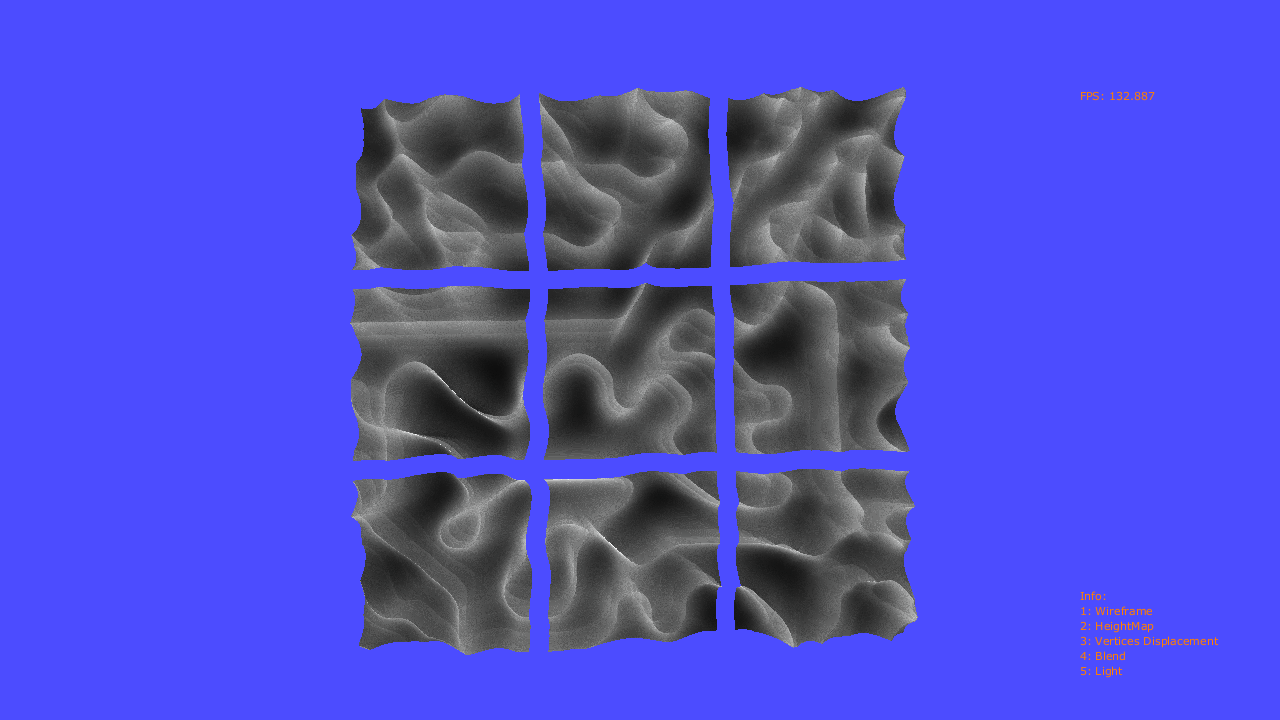
\includegraphics[width=0.6\linewidth]{img/caps/grid.png}}
	\caption{\label{fig:resultados:grid} \emph{Patchs} exibidos em um \emph{grid}.}
\end{figure}

Considerando o usu�rio inicialmente localizado no \emph{patch} central, ao mover-se para um \emph{patch} vizinho, o sistema ir� requisitar a gera�a� de novos \emph{patchs}, vizinhos a aqueles que est�o na borda do grid. O n�mero de vizinhos gerados, bem como a quantidade de vizinhos do \emph{patch} central s�o vari�veis do sistema, podendo ser adaptadas, pelo usu�rio, de acordo com o poder de processamento de sua m�quina.

Para garantir uma visualiza��o fluida do terreno, minimizando as interrup��es com a gera��o, o sistema proposto decidir� qual arquitetura (GPU ou CPU) ser� utilizada na gera��o dos \emph{patchs} a partir de uma vari�vel $\alpha$, que representa a porcentagem de gera��es que ocorrer�o na \emph{GPU}. $1 - \alpha$ representar�, portanto a porcentagem de gera��es na \emph{CPU}.

A Figura \ref{fig:geracao} mostra como se d� o fluxo de gera��o.

\begin{figure}[h]
	\center{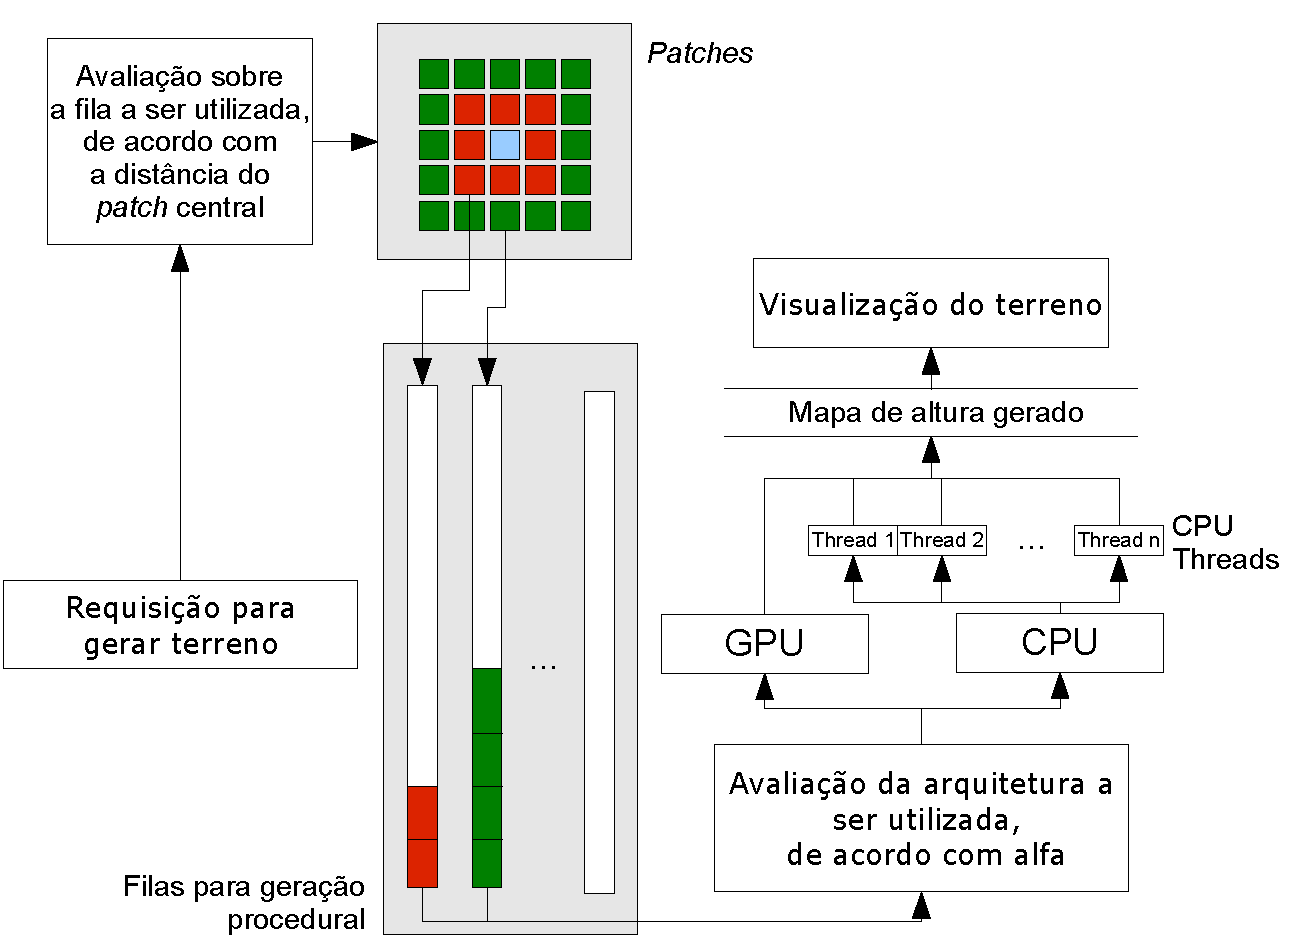
\includegraphics[width=1.0\linewidth]{img/geracao.pdf}}
	\caption{\label{fig:geracao} Fluxo da gera��o procedural.}
\end{figure}


As requisi��es por novos terrenos ser�o adicionadas a uma fila e uma pol�tica \emph{First In, First Out} (FIFO) ser� utilizada para decidir qual terreno ser� gerado. Como � poss�vel ver na Figura \ref{fig:geracao}, o n�mero de filas existentes no sistema ser� igual ao n�mero de vizinhos do \emph{patch} central. Dessa forma, � poss�vel decidir quais terrenos ser�o gerados a partir de sua dist�ncia do \emph{patch} central.

A \emph{thread} principal ficar� encarregada da requisi��o para gerar novos eventos, avalia��o da fila, avalia��o da arquitetura a ser utilizada as chamadas �s fun��es OpenGL. A gera��o na CPU ocorrer� em outras \emph{threads}, n�o a principal.



\subsection{O C�lculo de $\alpha$}

O valor da vari�vel $\alpha$ �, atualmente, uma vari�vel controlada manualmente pelo usu�rio.  A sua varia��o de acordo com a utiliza��o de cada arquitetura ser� um tema a ser abordado em trabalhos futuros.

Atualmente, a maior dificuldade para medir o tempo de gera��o tanto na GPU � a falta de um padr�o nas extens�es dispon�veis em OpenGL. A extens�o \textbf{GL\_EXT\_timer\_query} \cite{timerQuery}, por exemplo, s� est� dispon�vel em placas NVidia, algo que anularia a possibilidade da execu��o deste trabalho em placas ATI.

A utiliza��o de chamadas como \textbf{glFinish()} para sincronizar a CPU e a GPU e assim medir o tempo de gera��o dos terrenos poderia prejudicar a performance do sistema, j� que p�ra a execu��o da CPU enquanto todos os os comandos OpenGL n�o forem executados.

Uma outra op��o para a sincroniza��o seria a extens�o \textbf{GL\_NV\_fence} \cite{nvFence}, que oferece fun��es para sincroniza��o semelhantes ao \textbf{glFinish()} e \textbf{glFlush()}, por�m com um grau maior de controle sobre quais comandos OpenGL dever�o ser executados na chamada. Mais uma vez, por�m, a extens�o n�o est� dispon�vel para placas ATI.

\subsection{Gera��o}
Toda a gera��o dos terrenos na GPU � feita atrav�s de um \emph{fragment shader}, utilizando o ru�do Perlin como foi proposto em \cite{improvedPerlinNoise}. Como toda computa��o de \emph{shaders} fica limitada a geometrias ou texturas, foi preciso renderizar um quadrado utilizando as fun��es OpenGL, para que, dessa forma, fosse poss�vel aplicar os \emph{shaders} �s suas primitivas e iniciar os c�lculos necess�rios. O resultado da gera��o � renderizado em um \emph{framebuffer} \emph{off-screen}, que n�o � exibido na tela, atrav�s da exten��o FBO, que permite criar novos \emph{buffers}.

O c�lculo dos vetores gradientes, necess�rio no ru�do Perlin, � feito na CPU, apenas no in�cio do sistema, e depois � acessado no \emph{fragment shader} como uma textura 2D.

Como o mapa de altura � gerado na GPU, n�o h� qualquer tipo de perda de desempenho com a transfer�ncia entre a mem�ria RAM e a mem�ria da placa de v�deo. Um aspecto importante � que, durante a gera��o do mapa de altura, os valores das normais de cada v�rtice tamb�m s�o calculados.

A gera��o utilizando a CPU � feita utilizando o mesmo algoritmo implementado na GPU. Como o mapa de altura gerado reside na mem�ria principal, sua renderiza��o depender� da transfer�ncia para a mem�ria da placa de v�deo.


\subsection{Visualiza��o}
Com o mapa de altura gerado, o pr�ximo passo � exibir o terreno para o usu�rio, que � feito de forma id�ntica tanto para os terrenos gerados na GPU quanto para os gerados na CPU.

O passo inicial � a gera��o de uma malha (conjunto de v�rtices) de tamanho pr�-determinado, como mostra a Figura \ref{fig:malha}.

\begin{figure}[h]
	\center{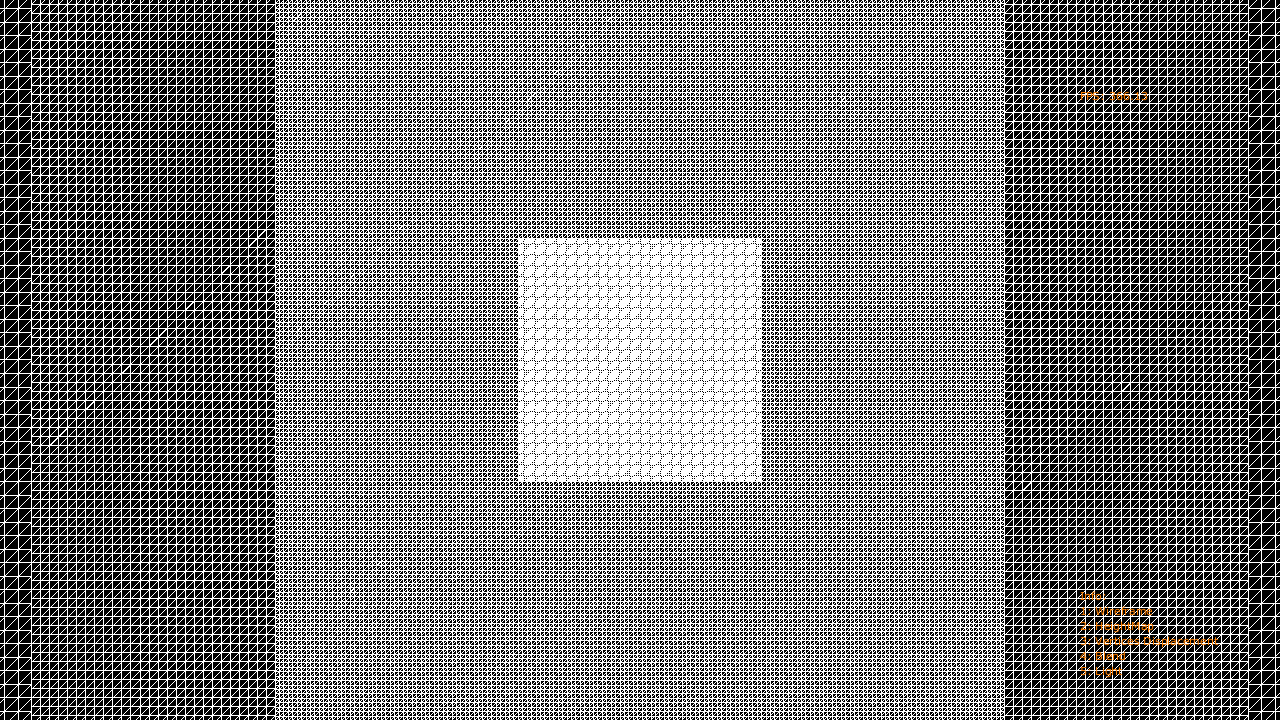
\includegraphics[width=0.5\linewidth]{img/caps/malha.png}}
	\caption{\label{fig:malha} Malha inicial para visualiza��o dos terrenos.}
\end{figure}

A malha � gerada de tal forma que um n�mero maior de v�rtices est� concentrado no centro. Quanto maior a dist�ncia, menor o n�mero de v�rtices presentes. Isto propicia uma maneira r�pida e f�cil de implementar um n�vel de detalhamento (quanto maior a dist�ncia do centro, menor ser� a necessidade de se renderizar o terreno em alta fidelidade).

Como a malha � gerada apenas uma �nica vez (no in�cio da execu��o), n�o � preciso criar repetidas malhas a medida que o jogador percorre o terreno. Apenas os mapas de altura de cada \emph{patch} s�o trocados, como mostra a Figura \ref{fig:texturas}

\begin{figure}[h]
	\center{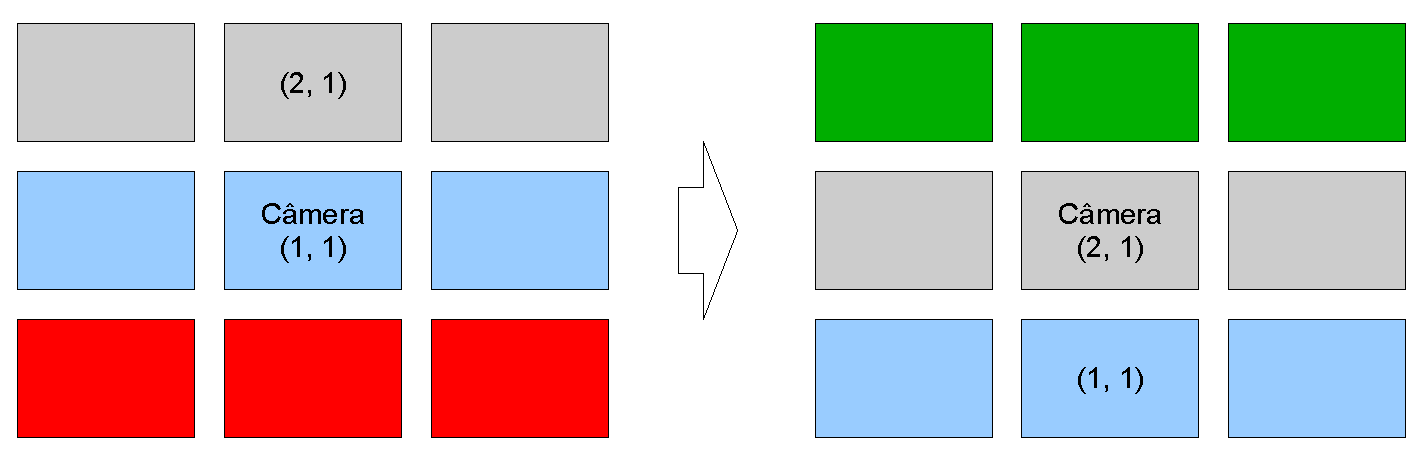
\includegraphics[width=0.8\linewidth]{img/texturas.pdf}}
	\caption{\label{fig:texturas} Movimenta��o da c�mera para um outro \emph{patchs}.}
\end{figure}

Na Figura \ref{fig:texturas} � poss�vel notar o deslocamento dos mapas de textura quando a c�mera move para o \emph{patch} superior ao (1,1). Para que haja uma transi��o, uma matriz de transla��o, com valores iguais ao tamanho do \emph{patch}, � feita e multiplicada � matriz respons�vel por renderizar todas as primitivas, resultando na transla��o de todos os \emph{patchs}. 

Este m�todo diminuiu a necessidade de implementa��o de um algoritmo de n�vel de detalhe mais robusto. Al�m disso, como sabemos o n�mero de v�rtices antecipadamente, a performance do aplicativo tem uma menor chance de sofrer quedas bruscas de rendimento.


\chapter{IMPLEMENTA��O}
\label{implementacao}

Os conhecimentos adquiridos ao longo desse trabalho permitiram a cria��o de um sistema capaz de gerar terrenos procedurais tanto na GPU quanto na CPU, e tamb�m permite a navega��o do usu�rio por tal terreno. Na Se��o \ref{sistema} ser� apresentado uma vis�o geral do sistema. As Se��es \ref{geracao} e \ref{visualizacao} mostrar�o como os terrenos s�o gerados e visualizados.



\section{Vis�o Geral do Sistema}
\label{sistema}

O sistema implementado neste trabalho teve como principal objetivo permitir a gera��o procedural de terrenos tanto na GPU quanto na CPU. A Figura \ref{fig:bibliotecas} apresenta as camadas do sistema, destacando as bibliotecas utilizadas (como � explicado a seguir).

\begin{figure}[H]
	\center{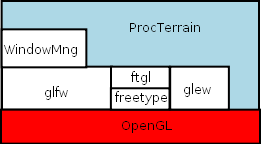
\includegraphics[width=0.3\linewidth]{img/bibliotecas.png}}
	\caption{\label{fig:bibliotecas} Camadas do sistema.}
\end{figure}

\begin{itemize}
	\item {\bf OpenGL}: \emph{API} gr�fica utilizada para a renderiza��o.
	\item {\bf glew}: Biblioteca para carregamento de extens�o do \emph{OpenGL}.
	\item {\bf glfw}: Biblioteca que facilita o tratamento de entradas e tamb�m cria��o de janelas.
	\item {\bf ftgl}: Biblioteca para a renderiza��o de textos.
	\item {\bf FreeType}: Biblioteca para renderiza��o de textos (depend�ncia do \emph{ftgl}).
	\item {\bf WindowMng}: Camada respons�vel por criar a tela e tratar os eventos de entrada.
	\item {\bf ProcTerrain}: Camada respons�vel por gerar e exibir os terrenos.
\end{itemize}

As camadas \emph{WindowMng} e \emph{ProcTerrain} foram implementadas neste trabalho. O \emph{WindowMng} tem como prop�sito simular a camada de um aplicativo gr�fico gen�rico (\emph{game}, simulador, etc.); desta forma, o sistema poder� ser posteriormente adaptado para funcionar em conjunto com outros aplicativos que possam ser desenvolvidos.

A Figura \ref{fig:arquitetura} apresenta em detalhes os m�dulos presentes nas camadas \emph{WindowMng} e \emph{ProcTerrain}. A seguir, uma explica��o sobre cada um dos m�dulos.

\begin{figure}[H]
	\center{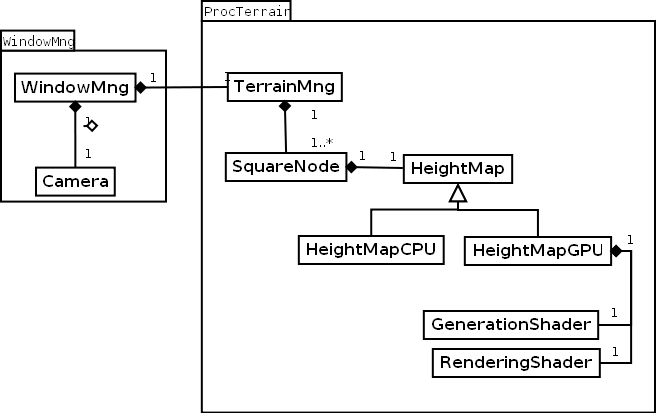
\includegraphics[width=0.5\linewidth]{img/arquitetura.png}}
	\caption{\label{fig:arquitetura} Diagrama com as principais classes do sistema implementado.}
\end{figure}

\begin{itemize}
	\item {\bf WindowMng}: Respons�vel por simular um aplicativo gr�fico gen�rico, e chamar os devidos \emph{callbacks} do pacote \emph{ProcTerrain}.
	\item {\bf Camera}: M�dulo que implementa uma c�mera controlada pelo jogador e navegando pelo mundo.
	\item {\bf TerrainMng}: M�dulo respons�vel por gerar e controlar os terrenos.
	\item {\bf SquareNode}: Nodo que representa uma fatia (\emph{patch}) do terreno.
	\item {\bf HeightMap}, {\bf HeightMapCPU} e {\bf HeightMapGPU}: M�dulos que implementam os mapas de altura dos terrenos gerados na CPU ou na GPU.
	\item {\bf GenerationShader}: \emph{Shader} respons�vel pela gera��o dos terrenos.
	\item {\bf RenderingShader}: \emph{Shader} respons�vel pela renderiza��o dos terrenos.
\end{itemize}


\section{Gera��o do Terreno}
\label{geracao}
Nesta se��o, ser� abordada a implementa��o da gera��o de terrenos, tanto na GPU, quanto na CPU. Os dois t�m, em comum, o algoritmo usado para a gera��o (\emph{Ridged multifractal noise}, descrito na Se��o \ref{ridged}).

O terreno geral � dividido em terrenos menores (chamados \emph{patchs}), como mostra o \emph{grid} da Figura \ref{fig:resultados:grid}:

\begin{figure}[H]
	\center{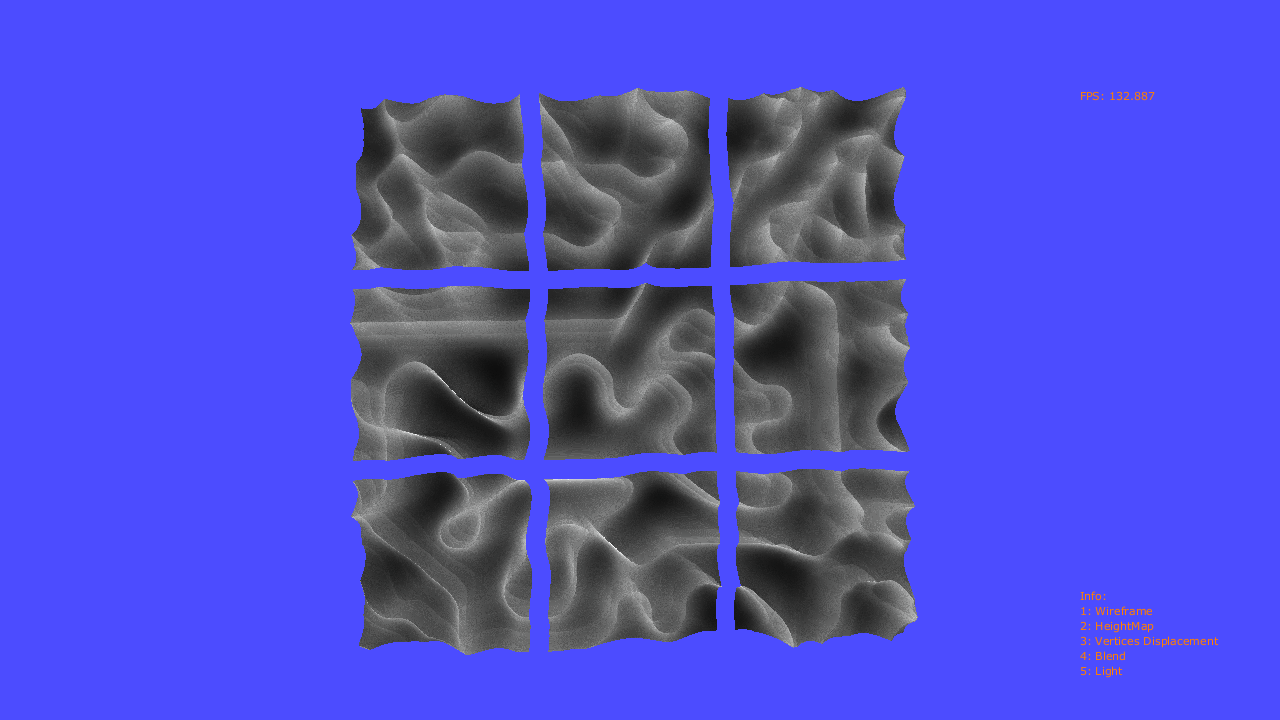
\includegraphics[width=0.5\linewidth]{img/caps/grid.png}}
	\caption{\label{fig:resultados:grid} \emph{Patchs} exibidos em um \emph{grid}.}
\end{figure}

Considerando o usu�rio inicialmente localizado no \emph{patch} central, ao mover-se para um \emph{patch} vizinho, o sistema ir� requisitar a gera�a� de novos \emph{patchs}, vizinhos a aqueles que est�o na borda do grid. O n�mero de vizinhos gerados, bem como a quantidade de vizinhos do \emph{patch} central s�o vari�veis do sistema, podendo ser adaptadas, pelo usu�rio, de acordo com o poder de processamento de sua m�quina.


\subsection{Gera��o do Terreno na GPU}
Toda a gera��o dos terrenos na GPU � feita atrav�s de um \emph{fragment shader}. Como toda computa��o de \emph{shaders} fica limitada a geometrias ou texturas, foi preciso renderizar um quadrado utilizando as fun��es OpenGL, para que, dessa forma, fosse poss�vel aplicar os \emph{shaders} �s suas primitivas e iniciar os c�lculos necess�rios. O resultado da gera��o � renderizado em um \emph{framebuffer} \emph{off-screen}, que n�o � exibido na tela, atrav�s da exten��o FBO, que permite criar novos \emph{buffers}.

O c�lculo dos vetores gradientes, necess�rio no ru�do Perlin, � feito na CPU, apenas no in�cio do sistema, e depois � acessado no \emph{fragment shader} como uma textura 2D.

A Figura \ref{fig:resultados:heightmap} apresenta o resultado da gera��o, visto como um mapa de altura.

\begin{figure}[H]
	\center{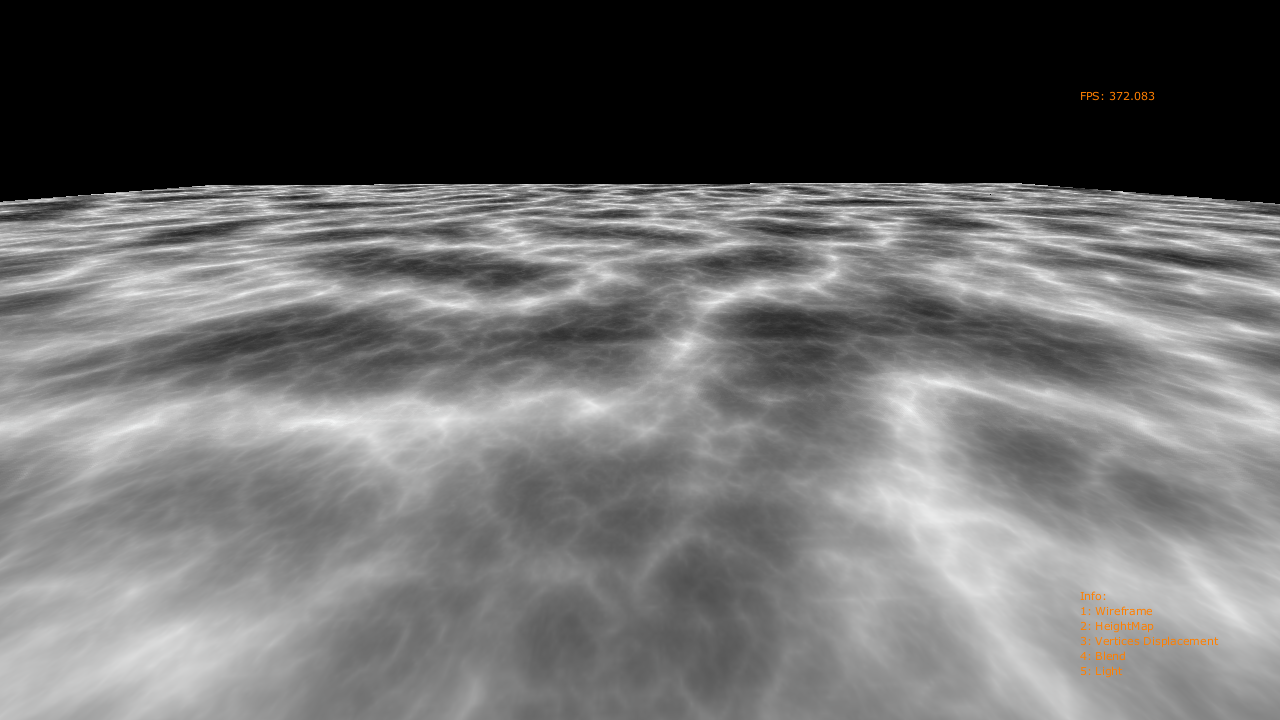
\includegraphics[width=0.5\linewidth]{img/caps/heightmap.png}}
	\caption{\label{fig:resultados:heightmap} Mapa de altura gerado pelo \emph{shader}.}
\end{figure}

Como o mapa de altura � gerado na GPU, n�o h� qualquer tipo de perda de desempenho com a transfer�ncia entre a mem�ria RAM e a mem�ria da placa de v�deo. Um aspecto importante � que, durante a gera��o do mapa de altura, os valores das normais de cada v�rtice tamb�m s�o calculados.



\subsection{Gera��o do Terreno na CPU}
A gera��o na CPU � feita de maneira tradicional. Uma matrix com o tamanho da textura do mapa de altura � preenchida de acordo com o algoritmo \emph{Ridged multifractal noise}, e posteriormente enviada para a mem�ria da GPU.



\section{Visualiza��o do Terreno}
\label{visualizacao}
Com o mapa de altura gerado, o pr�ximo passo � exibir o terreno para o usu�rio, que � feito de forma id�ntica tanto para os terrenos gerados na GPU quanto para os gerados na CPU.

O passo inicial � a gera��o de uma malha (conjunto de v�rtices) de tamanho pr�-determinado, como mostra a Figura \ref{fig:malha}.

\begin{figure}[H]
	\center{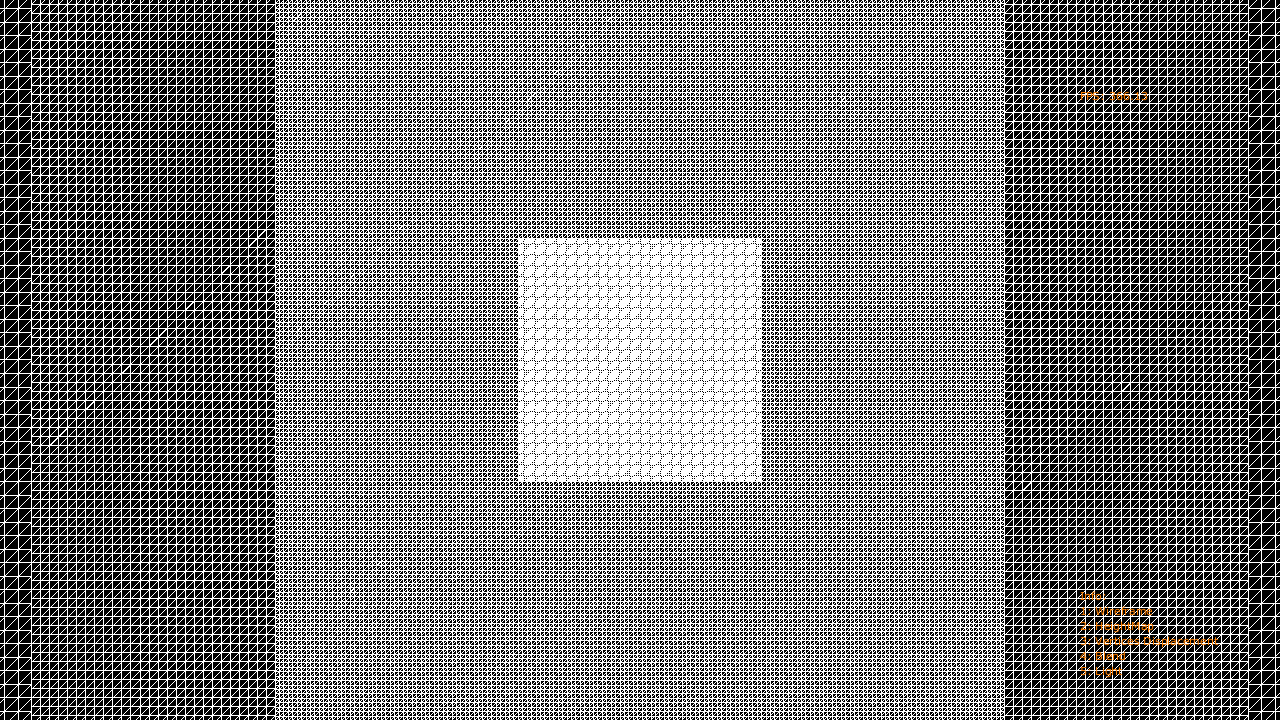
\includegraphics[width=0.5\linewidth]{img/caps/malha.png}}
	\caption{\label{fig:malha} Malha inicial para visualiza��o dos terrenos.}
\end{figure}

A malha � gerada de tal forma que um n�mero maior de v�rtices est� concentrado no centro. Quanto maior a dist�ncia, menor o n�mero de v�rtices presentes. Isto propicia uma maneira r�pida e f�cil de implementar um n�vel de detalhamento (quanto maior a dist�ncia do centro, menor ser� a necessidade de se renderizar o terreno em alta fidelidade).

Como a malha � gerada apenas uma �nica vez (no in�cio da execu��o), n�o � preciso criar repetidas malhas a medida que o jogador percorre o terreno. Apenas os mapas de altura de cada \emph{patch} s�o trocados, como mostra a Figura \ref{fig:texturas}

\begin{figure}[H]
	\center{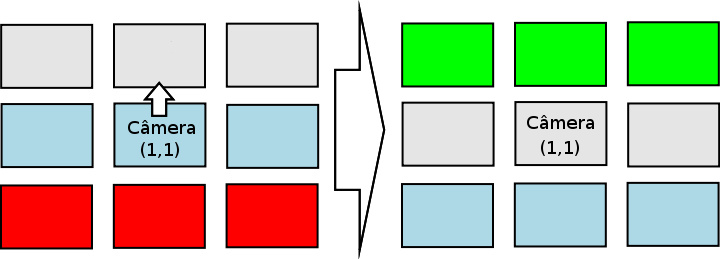
\includegraphics[width=0.8\linewidth]{img/texturas.png}}
	\caption{\label{fig:texturas} Movimenta��o da c�mera para um outro \emph{patchs}.}
\end{figure}

Na Figura \ref{fig:texturas} � poss�vel notar o deslocamento dos mapas de textura quando a c�mera move para o \emph{patch} superior ao (1,1). Para que haja uma transi��o, uma matriz de transla��o, com valores iguais ao tamanho do \emph{patch}, � feita e multiplicada � matriz \emph{MODELVIEW}, respons�vel por renderizar todas as primitivas, resultando na transla��o de todos os \emph{patchs}. 

Este m�todo diminuiu a necessidade de implementa��o de um algoritmo de n�vel de detalhe mais robusto. Al�m disso, como sabemos o n�mero de v�rtices antecipadamente, a performance do aplicativo tem uma menor chance de sofrer quedas bruscas de rendimento.

Ap�s a gera��o dos v�rtices, as texturas com os mapas de altura gerados proceduralmente s�o aplicados � malha. Um \emph{vertex shader} l� ent�o a altura presente no mapa e desloca a posi��o de \emph{z} do v�rtice correspondente na malha.

A cor de cada fragmento � calculada a partir de quatro diferentes texturas, simulando areia, grama, pedras e neve. A participa��o de cada uma delas na cor final depender� da altura do v�rtice correspondente do fragmento. Para pontos mais altos, a textura de neve ser� predominante e, pontos mais baixos, ser�o cobertos pela textura de grama. Entre esses pontos, haver� uma mistura das outras texturas.




\section{Testes}
\label{testes}

Para comprovar a efici�ncia do sistema, foi feito um teste que consiste na navega��o por um trajeto constante pelo terreno gerado proceduralmente, durante 30 segundos. O teste foi executado para cinco valores diferentes de $\alpha$: 1.0 (gera��o totalmente na GPU), 0.7, 0.4, 0.0 (gera��o totalmente na CPU).


\begin{figure}[h]
	\center{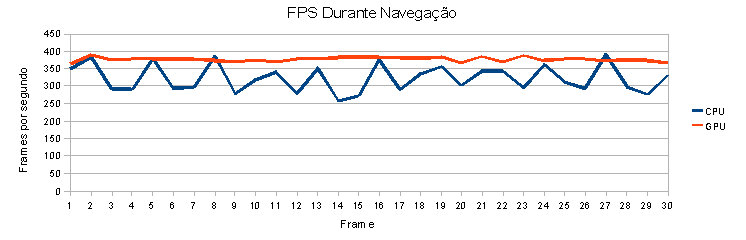
\includegraphics[width=0.9\linewidth]{img/tempoFPS.png}}
	\caption{\label{fig:fps} Gr�fico com o FPS na navega��o pelo mundo durante 30 segundos.}
\end{figure}
\section{Conclus�o e Trabalhos Futuros}
\label{conclusao}

Os resultados obtidos na gera��o procedural de terrenos na GPU mostram o poder de processamento das placas gr�ficas em rela��o �s CPU. A op��o de se gerar nas duas arquiteturas mostra-se promissora, principalmente considerando a utiliza��o do sistema acoplado a um \emph{game} ou simulador. Como haver� inevitavelmente outras tarefas sendo executadas (\emph{path-finding}, sombras, HDR), a possibilidade de se migrar a carga de trabalho envolvida na gera��o procedural pode ser bastante vantajosa.

Como trabalho futuro, espera-se encontrar uma estrat�gia eficiente para o c�lculo de $\alpha$. Dessa forma, a gera��o procedural poder� ser balanceada automaticamente entre as diferentes arquiteturas utilizadas (CPU e GPU).

O sistema foi implementado sempre tendo em mente a sua utiliza��o acoplada a outras aplicativos. Assim, adot�-lo em um \emph{game} ou simulador demandaria pouco esfor�o.




% An example of a floating figure using the graphicx package.
% Note that \label must occur AFTER (or within) \caption.
% For figures, \caption should occur after the \includegraphics.
% Note that IEEEtran v1.7 and later has special internal code that
% is designed to preserve the operation of \label within \caption
% even when the captionsoff option is in effect. However, because
% of issues like this, it may be the safest practice to put all your
% \label just after \caption rather than within \caption{}.
%
% Reminder: the "draftcls" or "draftclsnofoot", not "draft", class
% option should be used if it is desired that the figures are to be
% displayed while in draft mode.
%
%\begin{figure}[!t]
%\centering
%\includegraphics[width=2.5in]{myfigure}
% where an .eps filename suffix will be assumed under latex, 
% and a .pdf suffix will be assumed for pdflatex; or what has been declared
% via \DeclareGraphicsExtensions.
%\caption{Simulation Results}
%\label{fig_sim}
%\end{figure}

% Note that IEEE typically puts floats only at the top, even when this
% results in a large percentage of a column being occupied by floats.


% An example of a double column floating figure using two subfigures.
% (The subfig.sty package must be loaded for this to work.)
% The subfigure \label commands are set within each subfloat command, the
% \label for the overall figure must come after \caption.
% \hfil must be used as a separator to get equal spacing.
% The subfigure.sty package works much the same way, except \subfigure is
% used instead of \subfloat.
%
%\begin{figure*}[!t]
%\centerline{\subfloat[Case I]\includegraphics[width=2.5in]{subfigcase1}%
%\label{fig_first_case}}
%\hfil
%\subfloat[Case II]{\includegraphics[width=2.5in]{subfigcase2}%
%\label{fig_second_case}}}
%\caption{Simulation results}
%\label{fig_sim}
%\end{figure*}
%
% Note that often IEEE papers with subfigures do not employ subfigure
% captions (using the optional argument to \subfloat), but instead will
% reference/describe all of them (a), (b), etc., within the main caption.


% An example of a floating table. Note that, for IEEE style tables, the 
% \caption command should come BEFORE the table. Table text will default to
% \footnotesize as IEEE normally uses this smaller font for tables.
% The \label must come after \caption as always.
%
%\begin{table}[!t]
%% increase table row spacing, adjust to taste
%\renewcommand{\arraystretch}{1.3}
% if using array.sty, it might be a good idea to tweak the value of
% \extrarowheight as needed to properly center the text within the cells
%\caption{An Example of a Table}
%\label{table_example}
%\centering
%% Some packages, such as MDW tools, offer better commands for making tables
%% than the plain LaTeX2e tabular which is used here.
%\begin{tabular}{|c||c|}
%\hline
%One & Two\\
%\hline
%Three & Four\\
%\hline
%\end{tabular}
%\end{table}


% Note that IEEE does not put floats in the very first column - or typically
% anywhere on the first page for that matter. Also, in-text middle ("here")
% positioning is not used. Most IEEE journals/conferences use top floats
% exclusively. Note that, LaTeX2e, unlike IEEE journals/conferences, places
% footnotes above bottom floats. This can be corrected via the \fnbelowfloat
% command of the stfloats package.



% trigger a \newpage just before the given reference
% number - used to balance the columns on the last page
% adjust value as needed - may need to be readjusted if
% the document is modified later
%\IEEEtriggeratref{8}
% The "triggered" command can be changed if desired:
%\IEEEtriggercmd{\enlargethispage{-5in}}

% references section

% can use a bibliography generated by BibTeX as a .bbl file
% BibTeX documentation can be easily obtained at:
% http://www.ctan.org/tex-archive/biblio/bibtex/contrib/doc/
% The IEEEtran BibTeX style support page is at:
% http://www.michaelshell.org/tex/ieeetran/bibtex/
\bibliographystyle{IEEEtran}
% argument is your BibTeX string definitions and bibliography database(s)
\bibliography{paper}
%
% <OR> manually copy in the resultant .bbl file
% set second argument of \begin to the number of references
% (used to reserve space for the reference number labels box)
%\begin{thebibliography}{1}

%\bibitem{IEEEhowto:kopka}
%H.~Kopka and P.~W. Daly, \emph{A Guide to \LaTeX}, 3rd~ed.\hskip 1em plus
%  0.5em minus 0.4em\relax Harlow, England: Addison-Wesley, 1999.

%\end{thebibliography}




% that's all folks
\end{document}


